This section discusses the results of pose evaluation module. 

\section{Pose Evaluation Results on Angles}

Figure \ref{fig:angles_good} shows the graphs for 4 different types of angles from a good performance of punch-block compared against benchmark angle features. A good performance means it is similar to benchmark performance, therefore, the angles too are similar with the benchmark angles. However, a bad performance means that the action is not properly performed and the user angles do not seem very similar to the benchmark angles, as shown in figure \ref{fig:angles_bad}. For an average performance, the angles show an average amount of similarity with the benchmark angle features as shown in \ref{fig:angles_average}. Table \ref{table:AngleScores} shows the angle similarity scores computed for good, average and bad performances, good similarity scores indicate a performance similar to benchmark, while average and low similarity scores indicate an average or incorrect performance in comparison to benchmark respectivrly. This proves that the pose evaluation module provides good results for angle similarity score calculation. 

Table \ref{table:angleClassification} shows the classification of angle features into categories good, average and bad. The system is able to correctly classify the angles from a good performance into category good, and the angles from an average performance into category average, however, it classifies angles from a bad performance into category average and not into category bad. 

\bigskip

\begin{table}
  \begin{adjustbox}{width=\columnwidth,center}
  \begin{tabular}{|c|c|c|c|c|c|c|}
    \hline
    Type of Performance & Video No. & \multicolumn{5}{c}{Scores}   \\
        \hline
        \hline
         {} & {} & Right Elbow & Left Elbow & Right Shoulder & Left Shoulder & Overall \\
        \hline
        \multirow{2}{*}{Good Videos} 
          & Video 4 & 80.25\% & 73.9\% & 83.9\% & 82.4\% & 80.13\%   \\ \cline{2-7}
          & Video 5 & 80.1\% & 78.1\% & 82.5\% & 79.4\% & 80\% \\ \cline{2-7}
          & Video 6 & 93.6\% & 78.2\% & 93.57\% & 71.4\% & 84.24\% \\ \cline{2-7}
          & Video 8 & 92.9\% & 74.5\% & 92.8\% & 66.9\% & 81.7\% \\ \cline{2-7}
          \hline

          \multirow{2}{*}{Average Videos} 
          & Video 1 & 77.28\% & 59.1\% & 77.9\% & 67.6\% & 70.5\%   \\ \cline{2-7}
          & Video 9 & 74.9\% & 55.4\% & 75.1\% & 72.6\% & 69.5\% \\ \cline{2-7}
          \hline

          \multirow{2}{*}{Bad Videos} 
          & Video 17 & 62.8\% & 64.7\% & 63.9\% & 60.1\% & 62.9\%   \\ \cline{2-7}
          & Video 14 & 76.4\% & 46.7\% & 73.6\% & 57.6\% & 63.6\% \\ \cline{2-7}
          \hline
  \end{tabular}
\end{adjustbox}
\caption{Angle Similarity Scores Computed For Good, Average and Bad Performances}
\label{table:AngleScores}
\end{table}

\begin{table}
  \centering
  \begin{tabular}{|c|c|c|}
    \hline
    Type of Performance & Video No. & Category of Angle Features   \\
        \hline
        \hline
        \multirow{2}{*}{Good Videos} 
          & Video 4 &  Good \\ \cline{2-3}
          & Video 5 &  Good \\ \cline{2-3}
          & Video 6 &  Good \\ \cline{2-3}
          & Video 8 &  Good \\ \cline{2-3}
          \hline

          \multirow{2}{*}{Average Videos} 
          & Video 1 &  Average  \\ \cline{2-3}
          & Video 9 &  Average  \\ \cline{2-3}
          \hline

          \multirow{2}{*}{Bad Videos} 
          & Video 17 &  Average  \\ \cline{2-3}
          & Video 14 &  Average  \\ \cline{2-3}
          \hline
  \end{tabular}
\caption{Classification of Angle Features}
\label{table:angleClassification}
\end{table}

\begin{figure}
    \subfigure[Angle Results on Video 4]{% 
      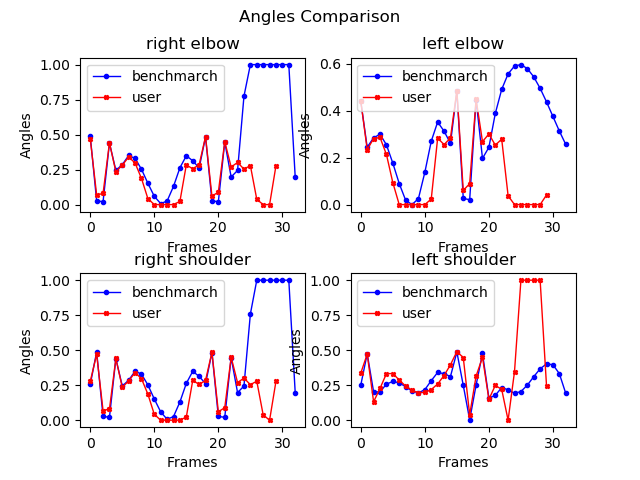
\includegraphics[scale=0.5]{images/graphs/angles_video4_good} \label{fig:video4_angles} 
    } 
   \quad 
    \subfigure[Angle Results on Video 5]{% 
      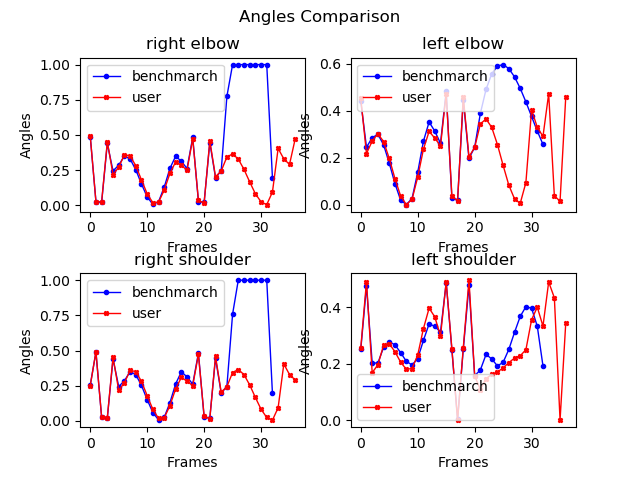
\includegraphics[scale=0.5]{images/graphs/angles_video5_good} \label{fig:video5_angles} 
    } \\
    \quad 
    \subfigure[Angle Results on Video 6]{% 
      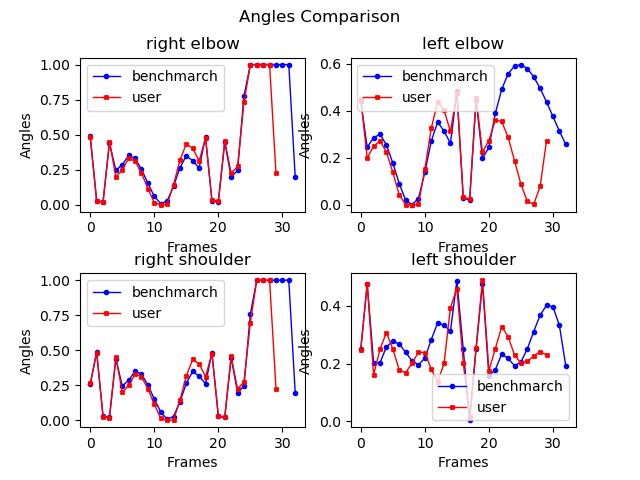
\includegraphics[scale=0.5]{images/graphs/angles_video6_good} \label{fig:video6_angles} 
    }
   \quad 
    \subfigure[Angle Results on Video 8]{% 
      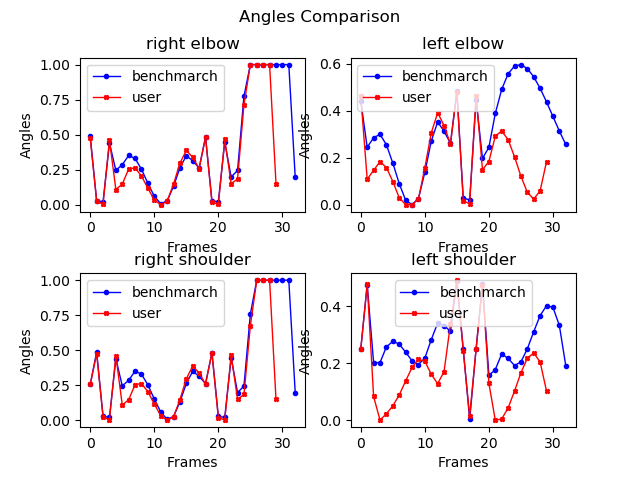
\includegraphics[scale=0.5]{images/graphs/angles_video8_good} \label{fig:video8_angles} 
    }
    \caption{Angle Results on Good Videos} 
    \centering
    \label{fig:angles_good}
  \end{figure}

  \begin{figure}
    \subfigure[Angle Results on Video 14]{% 
      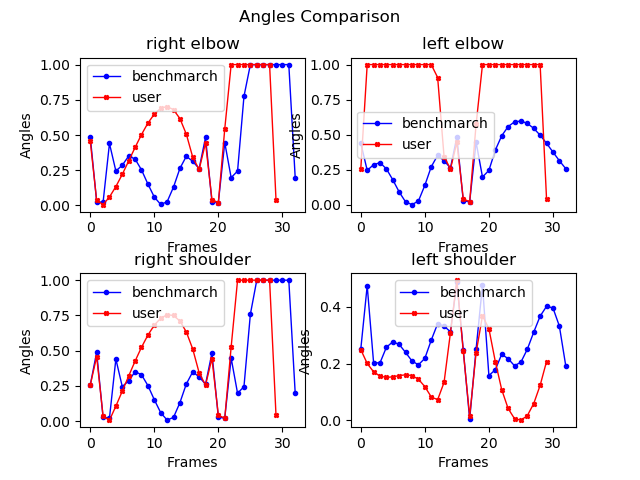
\includegraphics[scale=0.5]{images/graphs/angles_video14_bad} \label{fig:video14_angles} 
    } 
   \quad 
    \subfigure[Angle Results on Video 17]{% 
      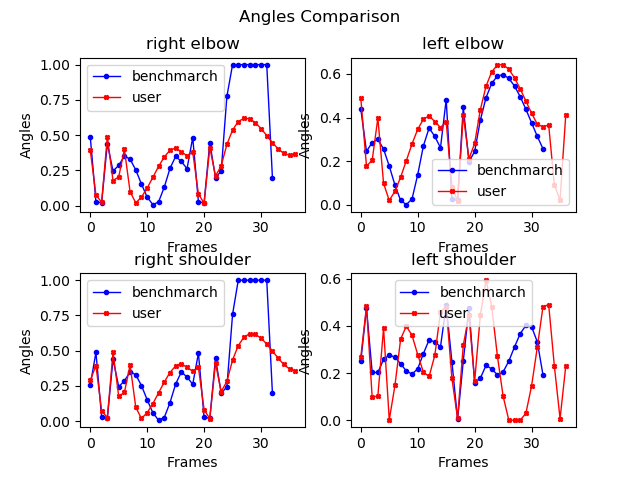
\includegraphics[scale=0.5]{images/graphs/angles_video17_bad} \label{fig:video17_angles} 
    } 
    \caption{Angle Results on Bad Videos} 
    \centering
    \label{fig:angles_bad}
  \end{figure}

  \begin{figure}
    \subfigure[Angle Results on Video 14]{% 
      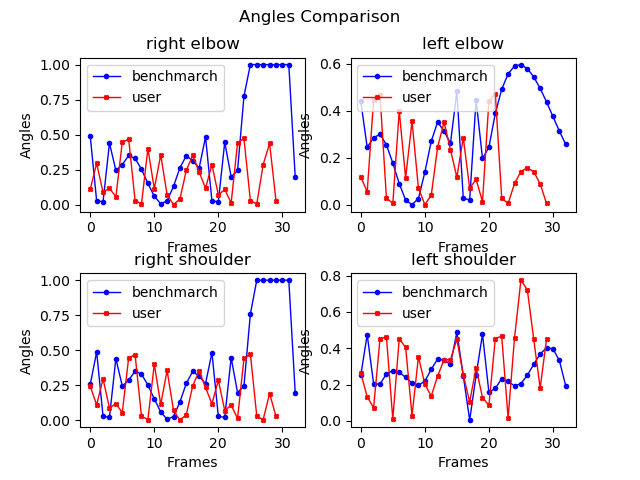
\includegraphics[scale=0.5]{images/graphs/angles_video1_average} \label{fig:video1_angles} 
    } 
   \quad 
    \subfigure[Angle Results on Video 17]{% 
      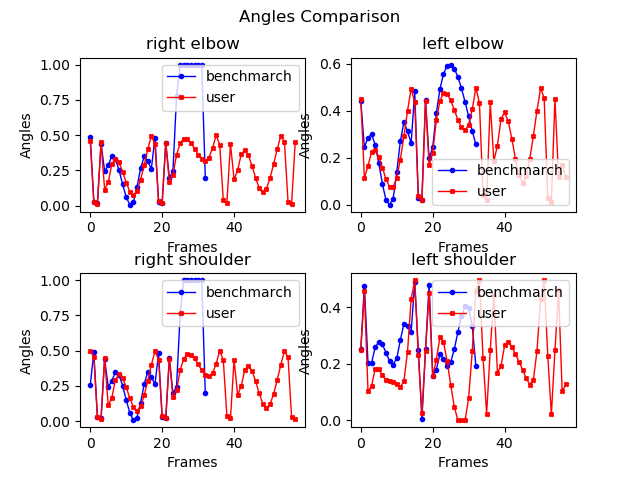
\includegraphics[scale=0.5]{images/graphs/angles_video9_average} \label{fig:video9_angles} 
    } 
    \caption{Angle Results on Average Videos} 
    \centering
    \label{fig:angles_average}
  \end{figure}

  \section{Pose Evaluation Results on Kinetic Energies}
  Figure \ref{fig:KE_results_good} shows the graphs for kinetic energies of 4 keypoints from good performances of punch-block compared against benchmark kinetic energy features of respective keypoints, the kinetic energy trends for both benchmark and user are roughly similar. A good performance means that it exerts kinetic energy roughly same or more than benchmark performance. However, a bad performance means that the action is not carried out with enough kinetic energy as shown in figure \ref{fig:KE_results_bad} where the trends for user's kinetic energy for almost all keypoints are significantly lower than benchmark kinetic energy trends. Figure \ref{fig:KE_results_average} shows the kinetic energy trends for average performances. Table \ref{table:KEScores} shows the kinetic energy similarity scores computed for good, average and bad performances, good similarity scores for kinetic energy indicate a performance carried out with similar energy as compared to benchmark, while low similarity scores for kinetic energy indicate an incorrect performance in comparison to benchmark with lower energy. This proves that the pose evaluation module provides good results for kinetic energy similarity score calculation. 

  Table \ref{table:KEClassification} shows the classification of kinetic energy features into categories good, average and bad. The system is able to correctly classify the kinetic energy features of most of the videos according to the original class of the entire performance. However, in our dataset because the videos are not produced by a professional, not all good videos have good kinetic energy levels, and not all bad videos have bad kinetic energy levels. Therefore, the incorrect classification is not a problem with the pose evaluation module, but with the dataset; see their respective figures for more clarity which show how much user and benchmark kinetic energy trends align together. 

  \begin{table}
    \centering
    \begin{tabular}{|c|c|c|}
      \hline
      Type of Performance & Video No. & Overall Scores   \\
          \hline
          \hline
          
          \multirow{2}{*}{Good Videos} 
            & Video 4 & 83\% \\ \cline{2-3}
            & Video 5 & 83.6\% \\ \cline{2-3}
            & Video 6 & 61.6\% \\ \cline{2-3}
            & Video 8 & 48.7\% \\ \cline{2-3}
            \hline

            \multirow{2}{*}{Average Videos} 
            & Video 1 & 67.3\% \\ \cline{2-3}
            & Video 9 & 57\% \\ \cline{2-3}
            \hline

            \multirow{2}{*}{Bad Videos} 
            & Video 14 & 62\% \\ \cline{2-3}
            & Video 17 & 81.6\% \\ \cline{2-3}
            \hline
    \end{tabular}
  \caption{Kinetic Energy Similarity Scores Computed For Good, Average and Bad Performances}
  \label{table:KEScores}
  \end{table}

  \begin{table}
    \centering
    \begin{tabular}{|c|c|c|}
      \hline
      Type of Performance & Video No. & Category of Kinetic Energy Features   \\
          \hline
          \hline
          \multirow{2}{*}{Good Videos} 
            & Video 4 &  Good \\ \cline{2-3}
            & Video 5 &  Good \\ \cline{2-3}
            & Video 6 &  Average \\ \cline{2-3}
            & Video 8 &  Bad \\ \cline{2-3}
            \hline
  
            \multirow{2}{*}{Average Videos} 
            & Video 1 &  Average  \\ \cline{2-3}
            & Video 9 &  Average  \\ \cline{2-3}
            \hline
  
            \multirow{2}{*}{Bad Videos} 
            & Video 17 &  Average  \\ \cline{2-3}
            & Video 14 &  Good  \\ \cline{2-3}
            \hline
    \end{tabular}
  \caption{Classification of Kinetic Energy Features}
  \label{table:KEClassification}
  \end{table}

  \begin{figure}
    \subfigure[Kinetic Energy Results on Video 4]{% 
      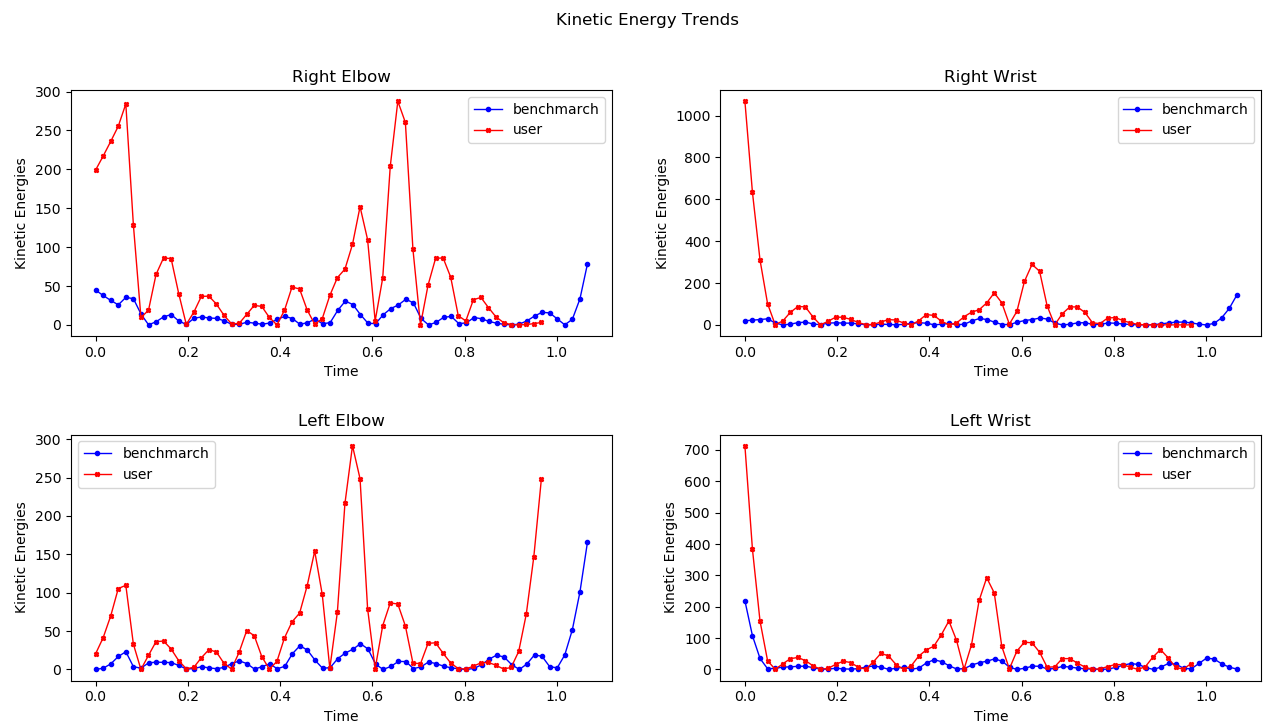
\includegraphics[scale=0.26]{images/graphs/KE_video4_good.png} \label{fig:video4_KE} 
    } 
   \quad 
    \subfigure[Kinetic Energy Results on Video 5]{% 
      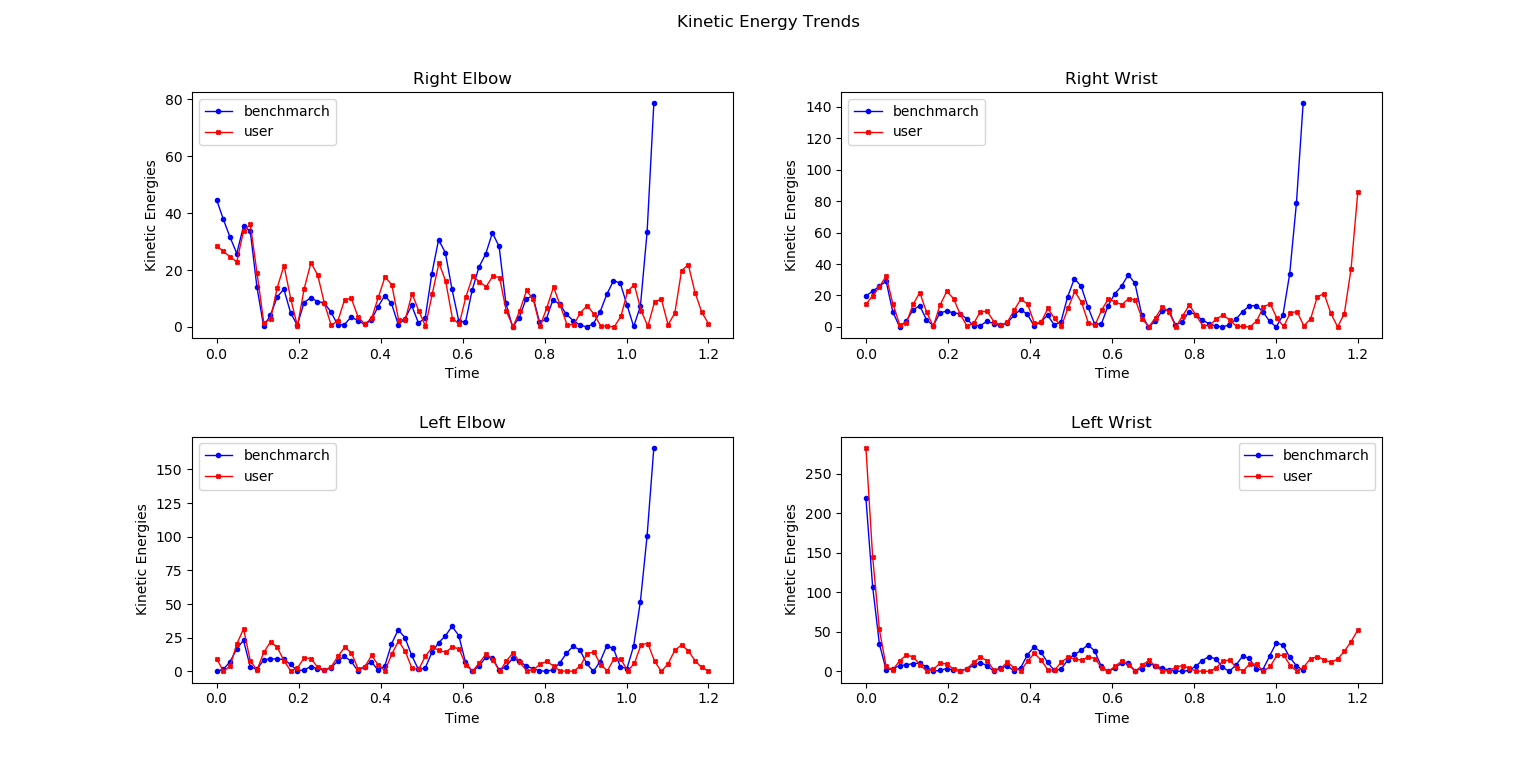
\includegraphics[scale=0.26]{images/graphs/KE_video5_good.png} \label{fig:video5_KE} 
    }  \\
    \subfigure[Kinetic Energy Results on Video 6]{% 
      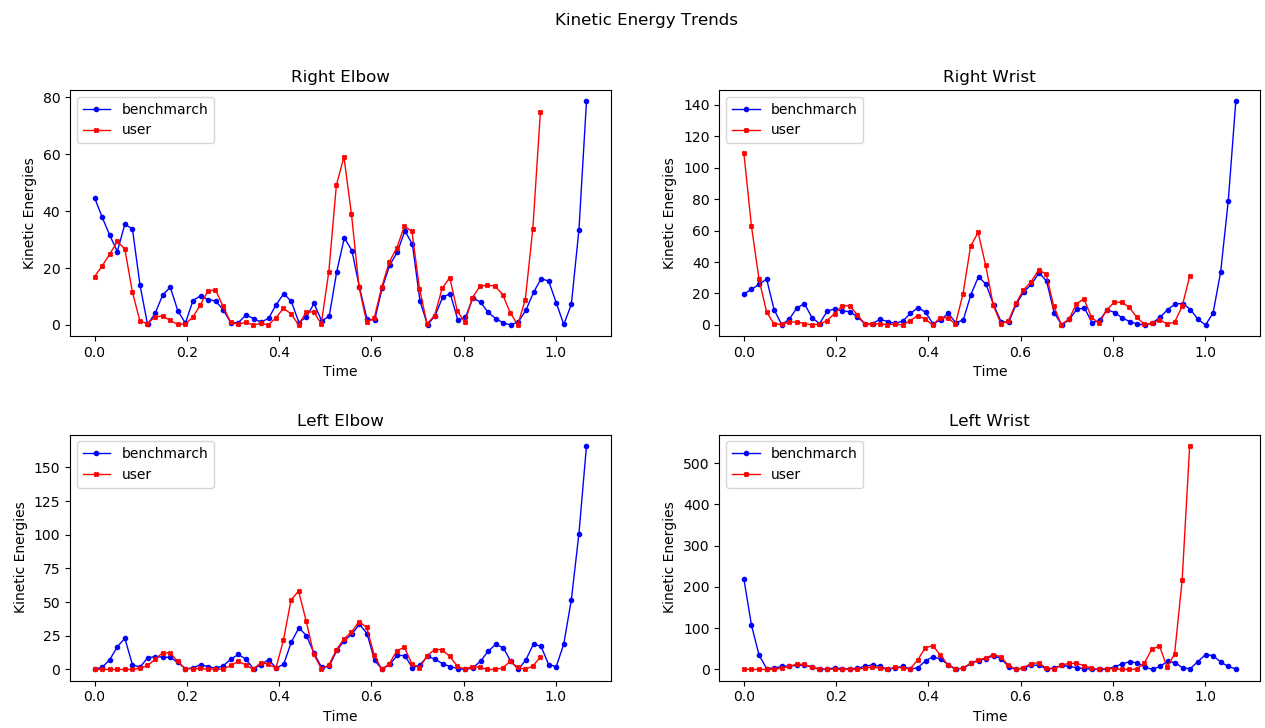
\includegraphics[scale=0.26]{images/graphs/KE_video6_good.png} \label{fig:video6_KE} 
    } 
   \quad 
    \subfigure[Kinetic Energy Results on Video 8]{% 
      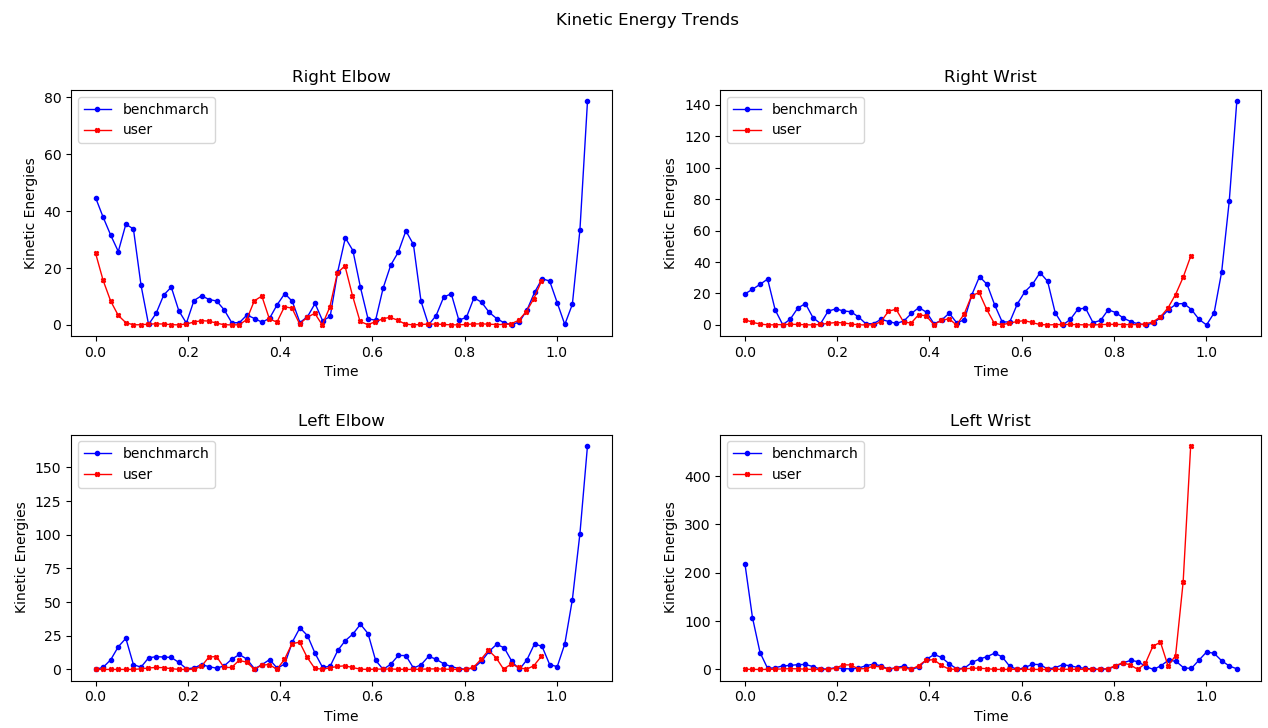
\includegraphics[scale=0.26]{images/graphs/KE_video8_good.png} \label{fig:video8_KE} 
    }
    \caption{Kinetic Energy Results on Good Videos} 
    \centering
    \label{fig:KE_results_good}
  \end{figure}

  \begin{figure}
    \subfigure[Kinetic Energy Results on Video 1]{% 
      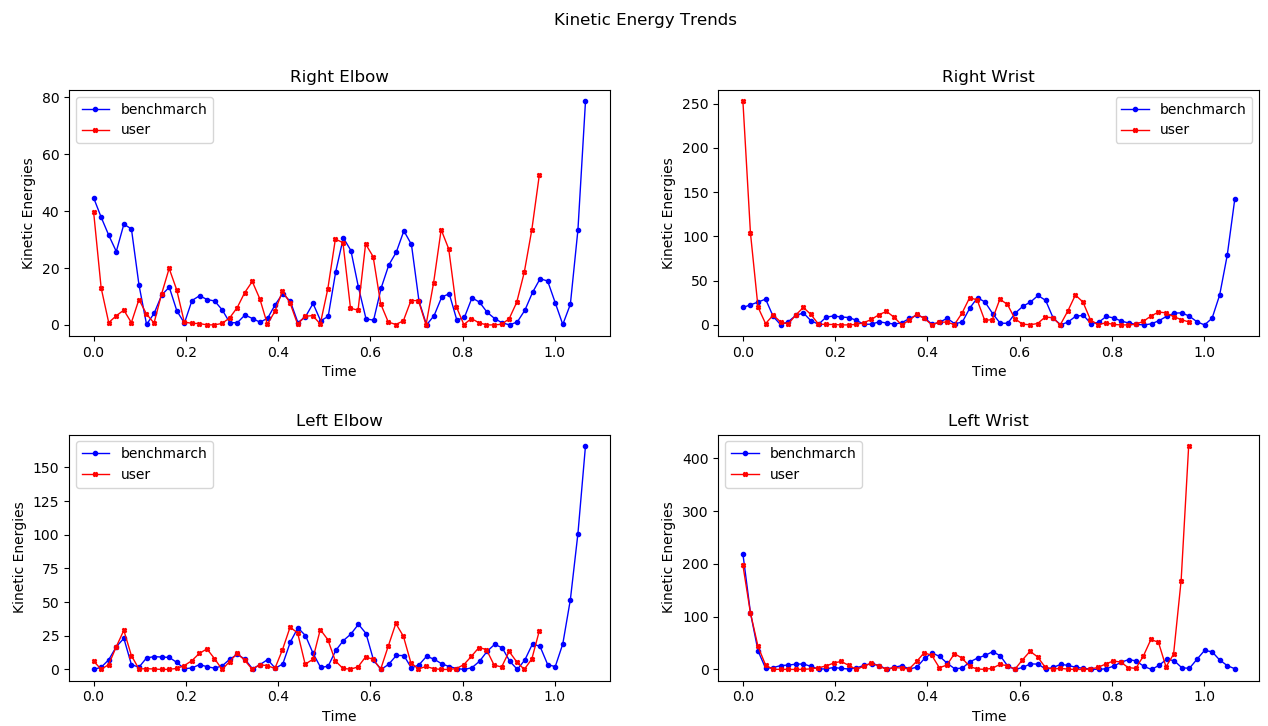
\includegraphics[scale=0.26]{images/graphs/KE_video1_average.png} \label{fig:video1_KE} 
    } 
   \quad 
    \subfigure[Kinetic Energy Results on Video 9]{% 
      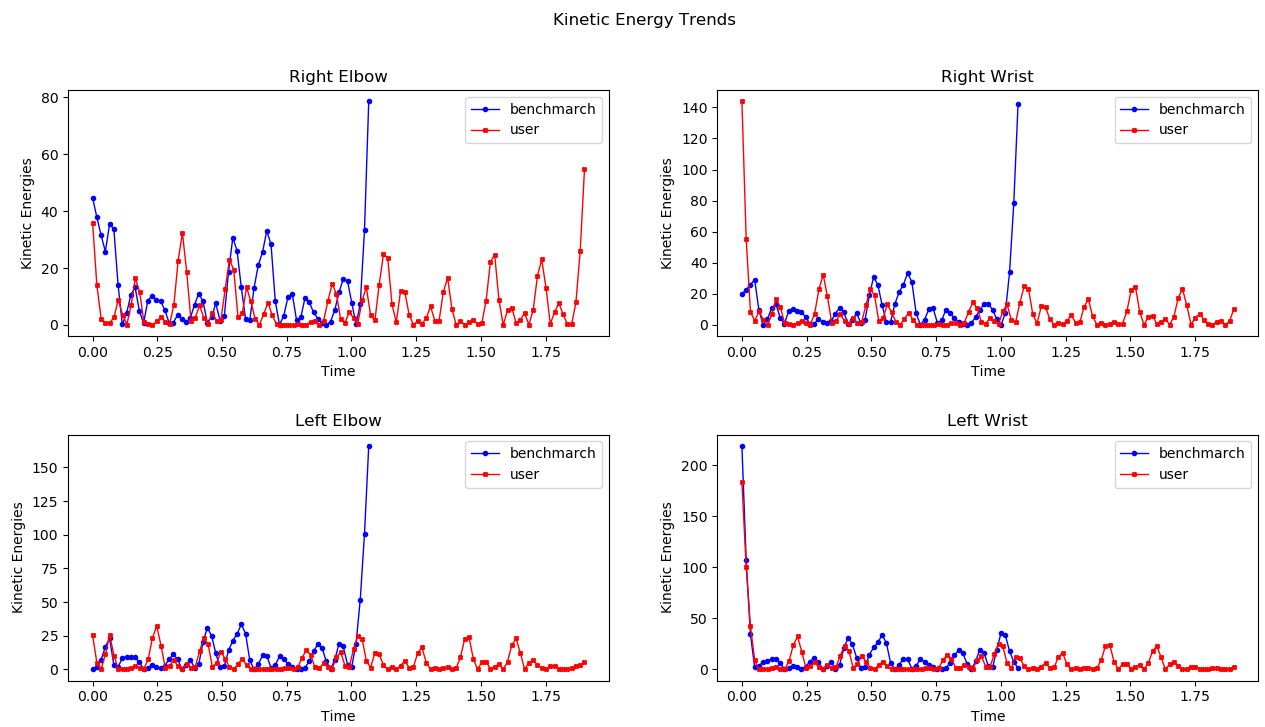
\includegraphics[scale=0.26]{images/graphs/KE_video9_average.png} \label{fig:video9_KE} 
    } 
    \caption{Kinetic Energy Results on Average Videos} 
    \centering
    \label{fig:KE_results_average}
  \end{figure}

  \begin{figure}
    \subfigure[Kinetic Energy Results on Video 14]{% 
      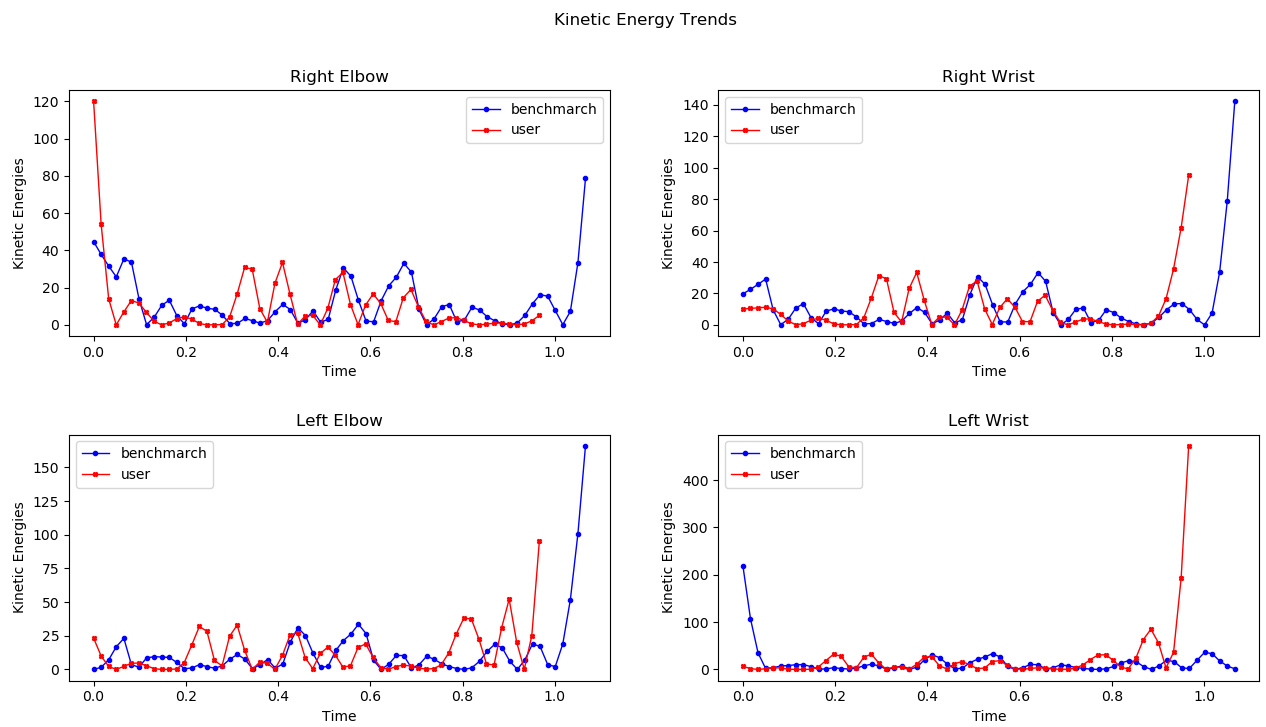
\includegraphics[scale=0.26]{images/graphs/KE_video14_bad.png} \label{fig:video14_KE} 
    } 
   \quad 
    \subfigure[Kinetic Energy Results on Video 17]{% 
      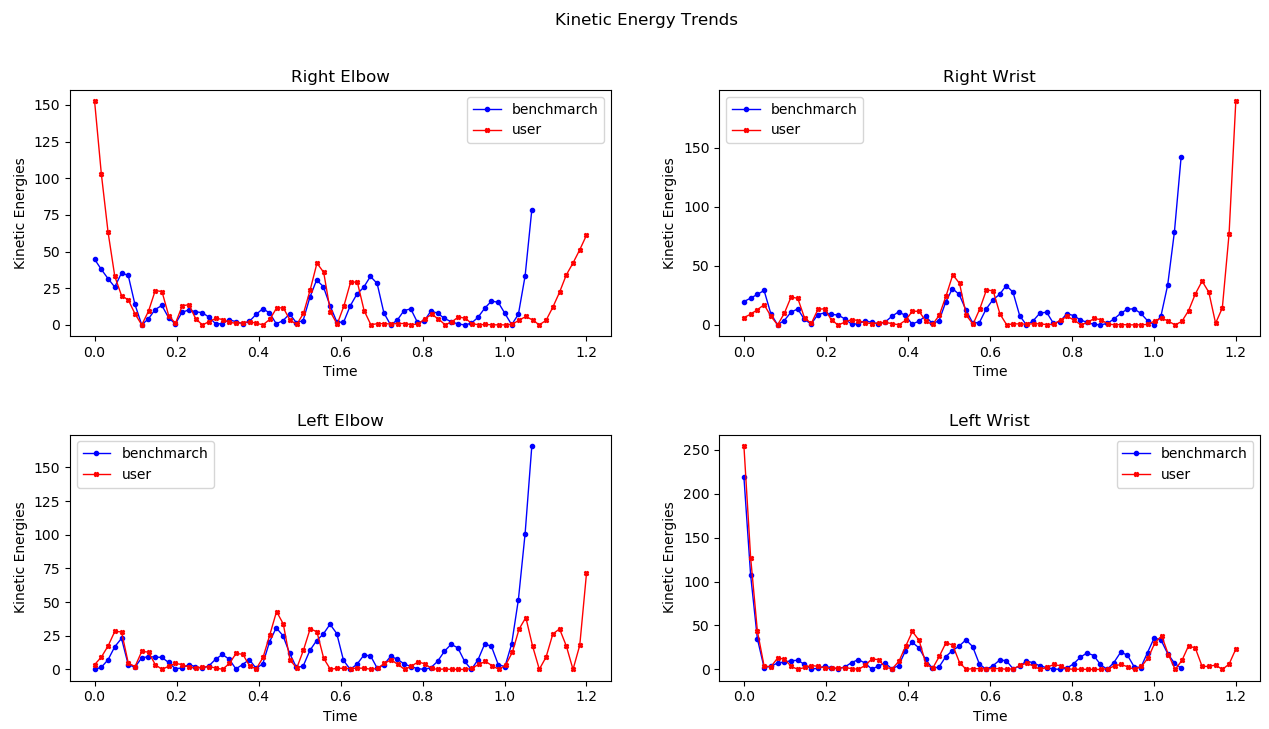
\includegraphics[scale=0.26]{images/graphs/KE_video17_bad.png} \label{fig:video17_KE} 
    } 
    \caption{Kinetic Energy Results on Bad Videos} 
    \centering
    \label{fig:KE_results_bad}
  \end{figure}

  \section{Pose Evaluation Results on Biomechanical Efficiency}
  Figure \ref{fig:AccDec_results_good} shows the graphs for acceleration and deceleration balance of wrist keypoints from good performances of punch-block compared against benchmark balance features of respective keypoints. A good punch-block performance means that the duration of acceleration is roughly balanced by duration of deceleration. However, a bad performance means that the duration of both is not balanced as shown in figure \ref{fig:AccDec_results_bad} where the duration of acceleration is much lesser than the duration of deceleration. \ref{fig:AccDec_results_average} shows the balance comparison for average performances. Table \ref{table:AccDecScores} shows the balance similarity scores computed for good, average and bad performances, good similarity scores for balance indicate a performance carried out with similar balance as compared to benchmark, while low similarity scores for balance indicate an incorrect performance in comparison to benchmark with lower energy. This proves that the pose evaluation module provides good results for balance similarity score calculation. 

  Table \ref{table:AccDecClassification} shows the classification of balance features into categories good, average and bad. The system is able to correctly classify the balance features for most of the videos according to the original class of the entire performance. However, in our dataset because the videos are not produced by a professional, not all good videos have good balance, and not all bad videos have bad balance. Therefore, the incorrect classification is not a problem with the pose evaluation module, but with the dataset.

\begin{table}
  \centering
  \begin{tabular}{|c|c|c|c|c|}
    \hline
    Type of Performance & Video No. & \multicolumn{3}{c}{Scores}   \\
        \hline
        \hline
         {} & {} & Right Wrist & Left Wrist & Overall \\
        \hline
        \multirow{2}{*}{Good Videos} 
          & Video 4 & 100\% & 100\% & 100\%  \\ \cline{2-5}
          & Video 5 & 16.69\% & 89.15\% & 52.9\% \\ \cline{2-5}
          & Video 6 & 100\% & 100\% & 100\%  \\ \cline{2-5}
          & Video 8 & 47\% & 88.7\% & 67.9\% \\ \cline{2-5}
          \hline

          \multirow{2}{*}{Average Videos} 
          & Video 1 & 92.8\% & 91.1\% & 91.9\% \\ \cline{2-5}
          & Video 9 & 17.12\% & 100\% & 58.5\% \\ \cline{2-5}
          \hline

          \multirow{2}{*}{Bad Videos} 
          & Video 17 & 78.9\% & 81.23\% & 80/1\%  \\ \cline{2-5}
          & Video 14 & 40.6\% & 39.7\% & 40.2\% \\ \cline{2-5}
          \hline
  \end{tabular}
\caption{Acceleration/Deceleration Balance Similarity Scores Computed For Good, Average and Bad Performances}
\label{table:AccDecScores}
\end{table}

\begin{table}
  \centering
  \begin{tabular}{|c|c|c|}
    \hline
    Type of Performance & Video No. & Category of Angle Features   \\
        \hline
        \hline
        \multirow{2}{*}{Good Videos} 
          & Video 4 &  Good \\ \cline{2-3}
          & Video 5 &  Bad \\ \cline{2-3}
          & Video 6 &  Good \\ \cline{2-3}
          & Video 8 &  Average \\ \cline{2-3}
          \hline

          \multirow{2}{*}{Average Videos} 
          & Video 1 &  Good  \\ \cline{2-3}
          & Video 9 &  Average  \\ \cline{2-3}
          \hline

          \multirow{2}{*}{Bad Videos} 
          & Video 17 &  Good  \\ \cline{2-3}
          & Video 14 &  Bad  \\ \cline{2-3}
          \hline
  \end{tabular}
\caption{Classification of Acceleration/Deceleration Balance Features}
\label{table:AccDecClassification}
\end{table}

\begin{figure}
  \centering
  \subfigure[Right Wrist]{% 
    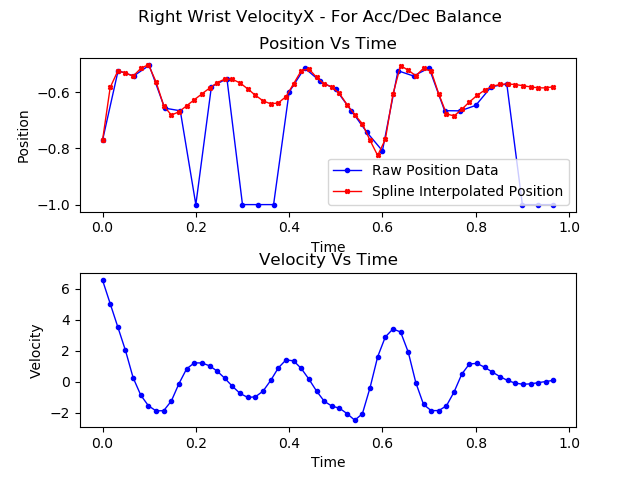
\includegraphics[scale=0.5]{images/graphs/accDecPhase_Video4_good_RWrist.png} \label{fig:video4_balance_right} 
  } 
 \quad 
  \subfigure[Left Wrist]{% 
    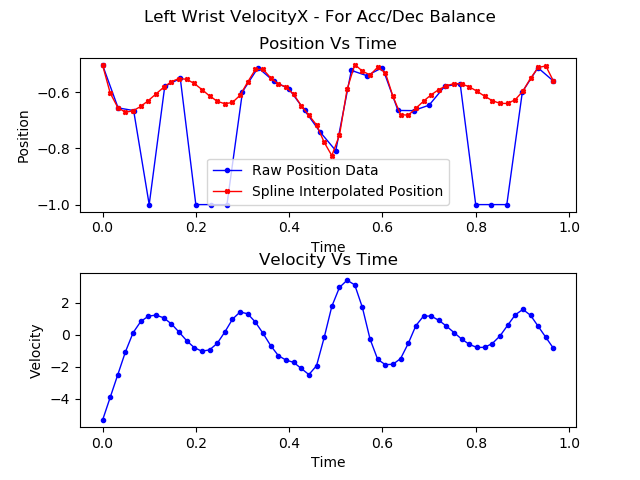
\includegraphics[scale=0.5]{images/graphs/accDecPhase_Video4_good_LWrist.png} \label{fig:video4_balance_left} 
  } 
  \caption{Acceleration Deceleration Balance Results on Good Video - 4}
  \label{fig:AccDec_results_good}
\end{figure}

\begin{figure}
  \centering
  \subfigure[Right Wrist]{% 
    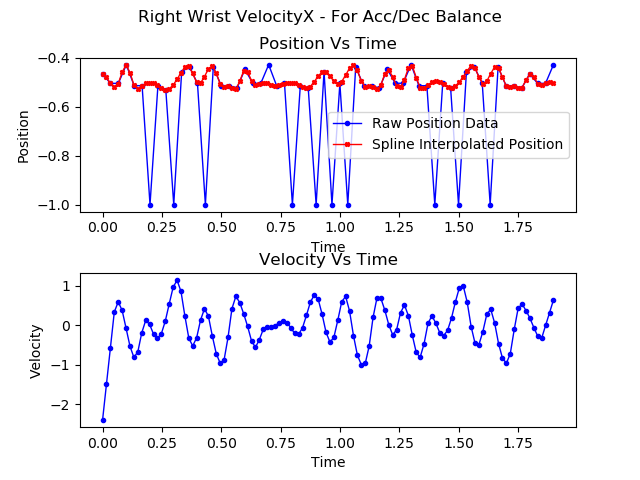
\includegraphics[scale=0.5]{images/graphs/accDecPhase_Video9_average_RWrist.png} \label{fig:video9_balance_right} 
  } 
 \quad 
  \subfigure[Left Wrist]{% 
    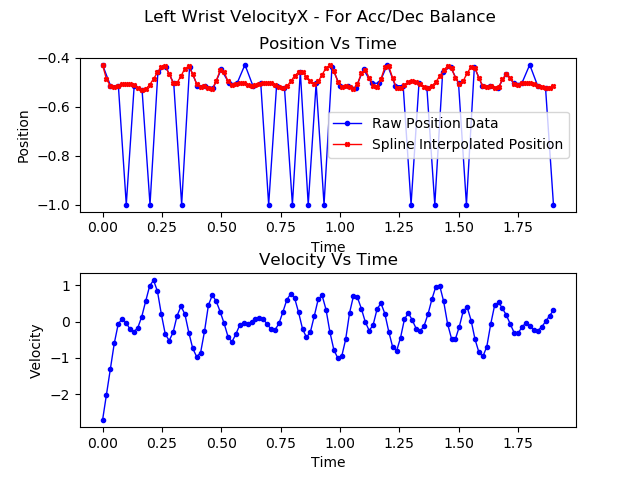
\includegraphics[scale=0.5]{images/graphs/accDecPhase_Video9_average_LWrist.png} \label{fig:video9_balance_left} 
  } 
  \caption{Acceleration Deceleration Balance Results on Average Video - 9}
  \label{fig:AccDec_results_average}
\end{figure}

\begin{figure}
  \centering
  \subfigure[Right Wrist]{% 
    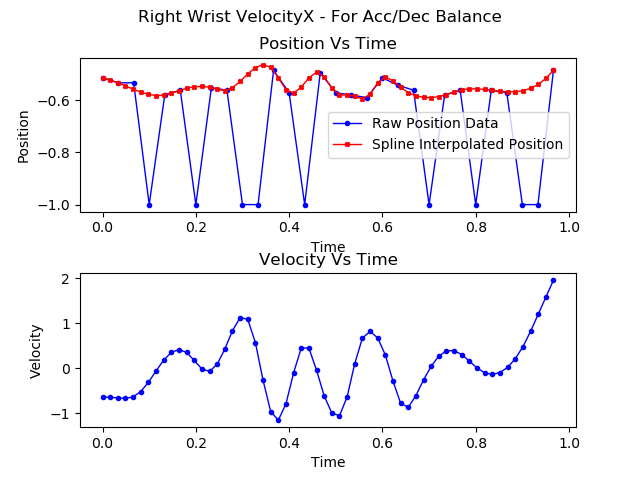
\includegraphics[scale=0.5]{images/graphs/accDecPhase_Video14_bad_RWrist.png} \label{fig:video14_balance_right} 
  } 
 \quad 
  \subfigure[Left Wrist]{% 
    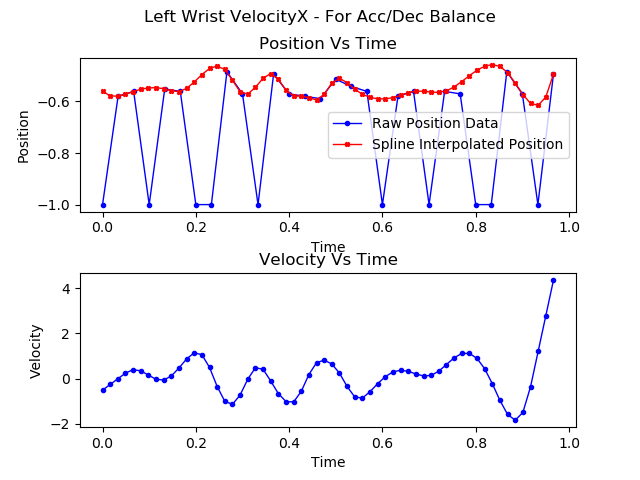
\includegraphics[scale=0.5]{images/graphs/accDecPhase_Video14_bad_LWrist.png} \label{fig:video14_balance_left} 
  } 
  \caption{Acceleration Deceleration Balance Results on Bad Video - 14}
  \label{fig:AccDec_results_bad}
\end{figure}


\section{Classification Results}

Apart from individual feature classification, we also classified the entire performance into categories 'good', 'average' or 'bad', see section \ref{section:classificationAndFeedback} for more details. Table \ref{table:overallClassification} shows the classification results of our pose evaluation module. The system almost correctly classifies all the good videos into good category, however, it is not able to distinguish between average and bad videos. One possible explanation for this behavior is the high similarity between average and bad videos dataset, and the system is not able to detect minor differences. If we merge the two categories, average and bad, then the system's accuracy for classification is $82.35\%$.

\begin{table}
  \centering
  \begin{tabular}{|c|c|c|}
    \hline
    Type of Performance & Video No. & Classification Category  \\
        \hline
        \hline
        \multirow{2}{*}{Good Videos} 
          & Video 2 &  Good \\ \cline{2-3}
          & Video 3 &  Average \\ \cline{2-3}
          & Video 4 &  Good \\ \cline{2-3}
          & Video 5 &  Good \\ \cline{2-3}
          & Video 6 &  Good \\ \cline{2-3}
          & Video 8 &  Good \\ \cline{2-3}
          \hline

          \multirow{2}{*}{Average Videos} 
          & Video 1 &  Average  \\ \cline{2-3}
          & Video 9 &  Average  \\ \cline{2-3}
          & Video 10 &  Average  \\ \cline{2-3}
          & Video 11 &  Average  \\ \cline{2-3}
          & Video 12 &  Average  \\ \cline{2-3}
          & Video 13 &  Average  \\ \cline{2-3}
          \hline

          \multirow{2}{*}{Bad Videos} 
          & Video 14 &  Average  \\ \cline{2-3}
          & Video 15 &  Bad  \\ \cline{2-3}
          & Video 16 &  Average  \\ \cline{2-3}
          & Video 17 &  Good  \\ \cline{2-3}
          & Video 18 &  Good  \\ \cline{2-3}
          \hline
  \end{tabular}
\caption{Classification of Entire Performance}
\label{table:overallClassification}
\end{table}




